\documentclass[12pt,a4paper]{article}
\usepackage[utf8]{inputenc}
\usepackage[spanish]{babel}
\usepackage{amsmath}
\usepackage{amsfonts}
\usepackage{amssymb}
\usepackage{graphicx}
\usepackage[left=2.5cm,right=2.5cm,top=3cm,bottom=3cm]{geometry}
\usepackage{xcolor}
\usepackage{listings}
\usepackage{tcolorbox}
\usepackage{hyperref}

% Configuración de colores para código
\definecolor{codegreen}{rgb}{0,0.6,0}
\definecolor{codegray}{rgb}{0.5,0.5,0.5}
\definecolor{codepurple}{rgb}{0.58,0,0.82}
\definecolor{backcolour}{rgb}{0.95,0.95,0.92}

\lstdefinestyle{mystyle}{
    backgroundcolor=\color{backcolour},   
    commentstyle=\color{codegreen},
    keywordstyle=\color{magenta},
    numberstyle=\tiny\color{codegray},
    stringstyle=\color{codepurple},
    basicstyle=\ttfamily\footnotesize,
    breakatwhitespace=false,         
    breaklines=true,                 
    captionpos=b,                    
    keepspaces=true,                 
    numbers=left,                    
    numbersep=5pt,                  
    showspaces=false,                
    showstringspaces=false,
    showtabs=false,                  
    tabsize=2
}
\lstset{style=mystyle}

\title{\textbf{Guía de Laboratorio 2}\\ \Large Detector de Temperatura con Pantalla y Alarma}
\author{Andrés Jaramillo - Andrea Zapata - Víctor Gonzales - Sergio Carmona - Daniela Nieto}
\date{\today}

\begin{document}

\maketitle

\section{Introducción}
En este proyecto se construye un termómetro digital inteligente utilizando Arduino. El sistema interactúa con un sensor de temperatura y humedad (DHT11), muestra los datos en tiempo real en una pantalla LCD I2C y programa una lógica de control que enciende un LED de advertencia cuando la temperatura supera los $28^\circ\text{C}$.

\section{Materiales y Ensamblaje del Circuito}
\begin{itemize}
    \item Placa Arduino Uno (o equivalente)
    \item Sensor de Temperatura y Humedad DHT11
    \item Pantalla LCD 16x2 con Módulo I2C
    \item LED rojo y Resistencia ($220\Omega - 330\Omega$)
    \item Protoboard y Jumpers
\end{itemize}

\begin{tcolorbox}[colback=red!5!white,colframe=red!75!black,title=Detalle de Pines]
\textbf{Sensor DHT11:} VCC a 5V, GND a GND, Señal al Pin Digital 2.\\
\textbf{Pantalla LCD I2C:} VCC a 5V, GND a GND, SDA al pin A4, SCL al pin A5.\\
\textbf{LED de Alarma:} Pin Digital 8 al Ánodo (mediante resistencia); GND al Cátodo.
\end{tcolorbox}

\begin{figure}[h]
    \centering
    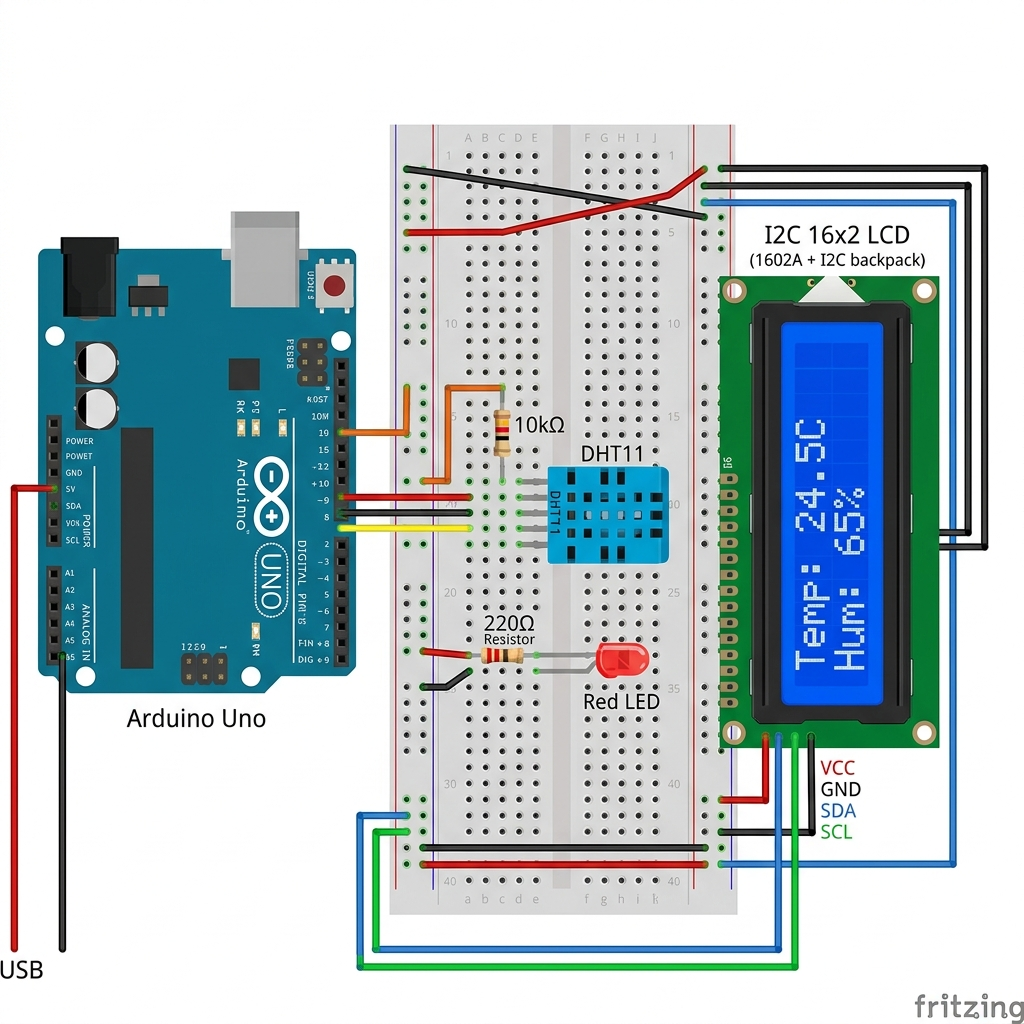
\includegraphics[width=0.7\textwidth]{circuito_temperatura.png}
    \caption{Diagrama del circuito del detector de temperatura.}
\end{figure}

\subsection{Fotos del Ensamblaje Real}
\begin{figure}[h]
    \centering
    \begin{minipage}{0.48\textwidth}
        \centering
        \includegraphics[width=\textwidth]{"Detector de Temperatura con Pantalla/WhatsApp Image 2026-05-15 at 12.49.25 PM.jpeg"}
        \caption{Conexión del sensor y pantalla.}
    \end{minipage}
    \hfill
    \begin{minipage}{0.48\textwidth}
        \centering
        \includegraphics[width=\textwidth]{"Detector de Temperatura con Pantalla/WhatsApp Image 2026-05-15 at 12.49.25 PM (1).jpeg"}
        \caption{Detalle del cableado I2C.}
    \end{minipage}
    \vspace{0.5cm}
    \begin{minipage}{0.48\textwidth}
        \centering
        \includegraphics[width=\textwidth]{"Detector de Temperatura con Pantalla/WhatsApp Image 2026-05-15 at 12.49.25 PM (2).jpeg"}
        \caption{Vista general del prototipo.}
    \end{minipage}
    \hfill
    \begin{minipage}{0.48\textwidth}
        \centering
        \includegraphics[width=\textwidth]{"Detector de Temperatura con Pantalla/WhatsApp Image 2026-05-15 at 12.49.26 PM.jpeg"}
        \caption{Prueba de funcionamiento.}
    \end{minipage}
\end{figure}

\section{Código Fuente}
\begin{lstlisting}[language=C++]
#include <Wire.h>
#include <LiquidCrystal_I2C.h>
#include <DHT.h>

#define DHTPIN 2       
#define DHTTYPE DHT11  
DHT dht(DHTPIN, DHTTYPE);

LiquidCrystal_I2C lcd(0x27, 16, 2);

const int pinLedAlarma = 8;
const float LIMITE_TEMPERATURA = 28.0; 

void setup() {
  Serial.begin(9600);
  pinMode(pinLedAlarma, OUTPUT);
  digitalWrite(pinLedAlarma, LOW);

  dht.begin();
  lcd.init();
  lcd.backlight();
  lcd.setCursor(0, 0);
  lcd.print("Iniciando...");
  delay(2000);
  lcd.clear();
}

void loop() {
  delay(2000);
  float h = dht.readHumidity();
  float t = dht.readTemperature();

  if (isnan(h) || isnan(t)) {
    lcd.setCursor(0, 0);
    lcd.print("Error de sensor!");
    return;
  }

  lcd.setCursor(0, 0);
  lcd.print("Temp: "); lcd.print(t, 1); lcd.print(" C   ");

  lcd.setCursor(0, 1);
  lcd.print("Hum:  "); lcd.print(h, 1); lcd.print(" %   ");

  if (t > LIMITE_TEMPERATURA) {
    digitalWrite(pinLedAlarma, HIGH);
  } else {
    digitalWrite(pinLedAlarma, LOW);
  }
}
\end{lstlisting}

\section{Pruebas y Resultados}
\begin{enumerate}
    \item Conecta el Arduino y sube el código.
    \item Verifica que la pantalla LCD muestre valores coherentes.
    \item Aplica calor al sensor y comprueba que el LED se encienda al cruzar el umbral de $28^\circ\text{C}$.
\end{enumerate}

\begin{figure}[h]
    \centering
    % \includegraphics[width=0.8\textwidth]{foto_funcionamiento.jpg}
    \caption{Sistema de monitoreo de temperatura en funcionamiento (Espacio para foto).}
\end{figure}

\end{document}
